
\cleardoublepage


\chapter{Northeast Beam Port Modeling}

% ------------------------------------------------------------------------------
\section{Introduction}

% ------------------------------------------------------------------------------
\section{Addition of Northeast Beam Port}


\subsection{Existing Model}

% introduce the idea of the model
% talk about the effort
In the summer of 2017, a reactor modeling effort was initiated at KSU.
% why it started
The goal of the effort was to produce, from the ground up, a python-based suite that would interpret geometric and material data related to KSU's Triga Mark II research reactor and produce input files for various transport codes.
% what has been produced so far
The model currently contains all of the major features from the actual reactor.
There are 85 fuel elements, containing fresh fuel, that are able to be automatically discretized axially, radially, and azimuthally into up to 10,000 cells.
The four control rods are also included, and a user may specify their exact position to match that of in-core experiments.
The central thimble, grid plates, and source location are all also included in the core model, which is surrounded by the graphite reflector.
Before the addition of the beam port, this is the furthest the model extended.
This model can be seen in \FIG{fig:existingyz} and \FIG{fig:existingxy}

% yz picture of the old reactor model
\begin{figure}[htb]
\centering
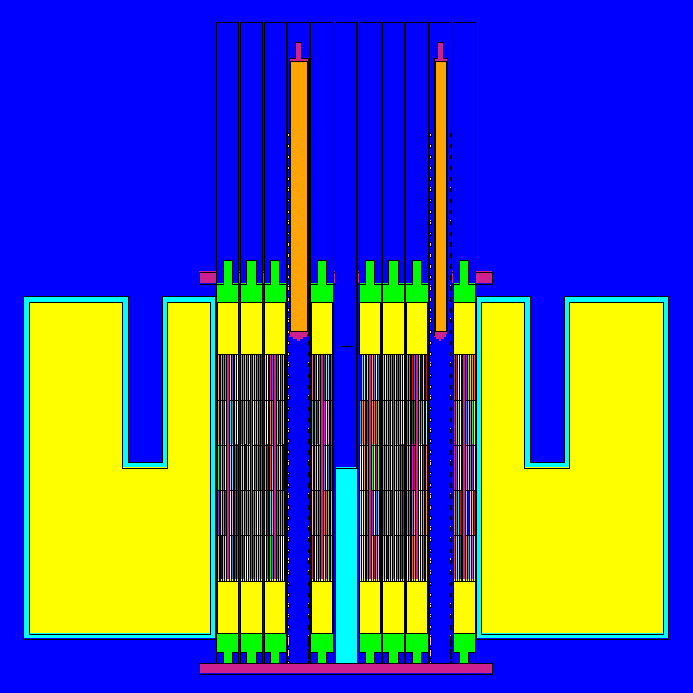
\includegraphics[height=3in]{tex/figures/existingyz.png}
\caption[Old Reactor Model $YZ$]{A $yz$ slice of the existing reactor model before the addition of the beam port.}
\label{fig:existingyz}
\end{figure}

% xy picture of the old reactor model
\begin{figure}[htb]
\centering
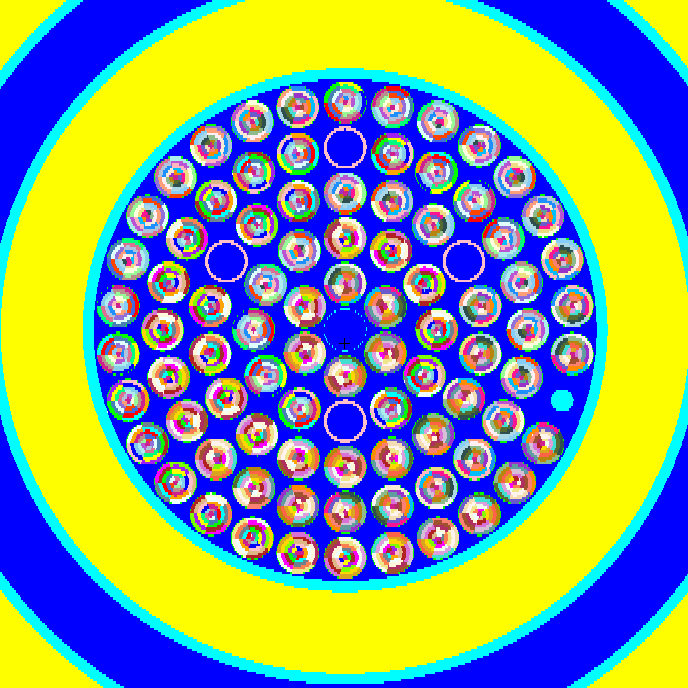
\includegraphics[height=3in]{tex/figures/existingxy.png}
\caption[Old Reactor Model $XY$]{An $xy$ slice of the existing reactor model before the addition of the beam port.}
\label{fig:existingxy}
\end{figure}


\subsection{The Beam Port Geometry}

% introduce
Using this model as a starting point, the northeast beam port (NEBP) was then added.
% what is the beam port
The NEBP, also known as the penetrating beam port or the fast beam port, is in essence, a large collimating cavity in the reactor's structure that allows neutrons to stream from the core to the outside of the reactor.
% purpose
The primary purpose of this is to provide a monodirectional neutron source, the strength of which can be scaled easily via reactor control.
This can be used for detector calibrations and testing, neutron imaging, or sample irradiation through neutron activation analysis.
The NEBP is unique in the fact that it penetrates the graphite reflector providing, in theory, the hardest neutron spectrum of the four beam ports at KSU.
This is due to the absence of significant moderating material between the fuel and the beam port.

% isometric view of the solidworks model of the beam port
\begin{figure}[htb]
\centering
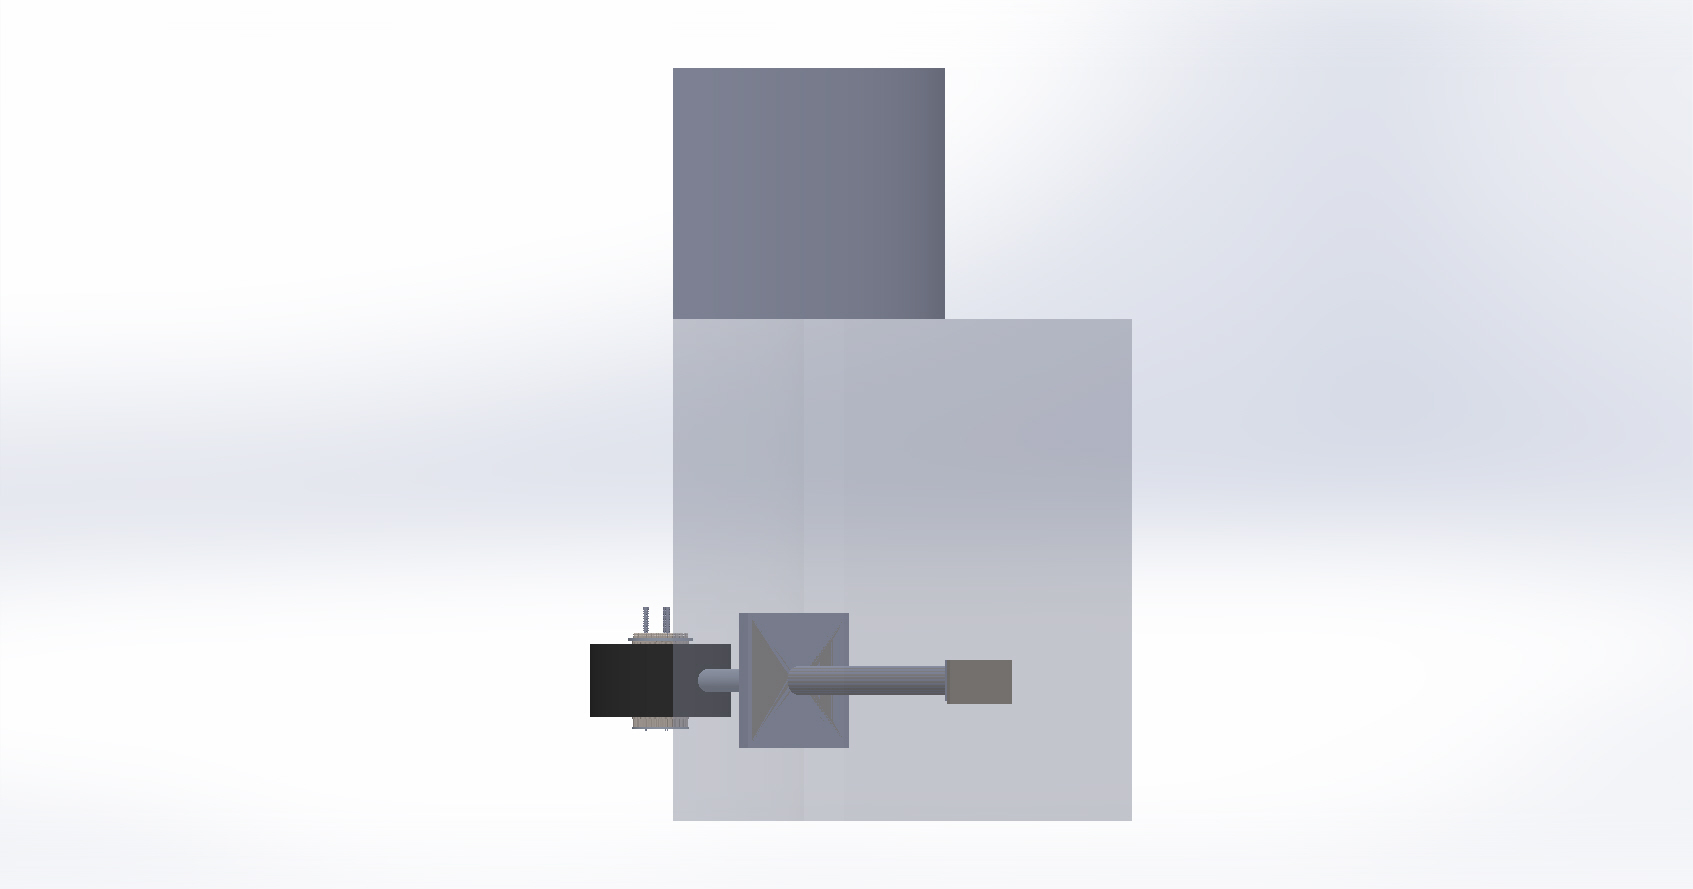
\includegraphics[height=3in]{tex/figures/solidworksangled.jpg}
\caption[Solidworks Angled NEBP]{An angled view of the NEBP with the reactor with a quarter section of the reactor structure.}
\label{fig:solidworksangled}
\end{figure}

% isometric view of the solidworks model of the beam port
\begin{figure}[htb]
\centering
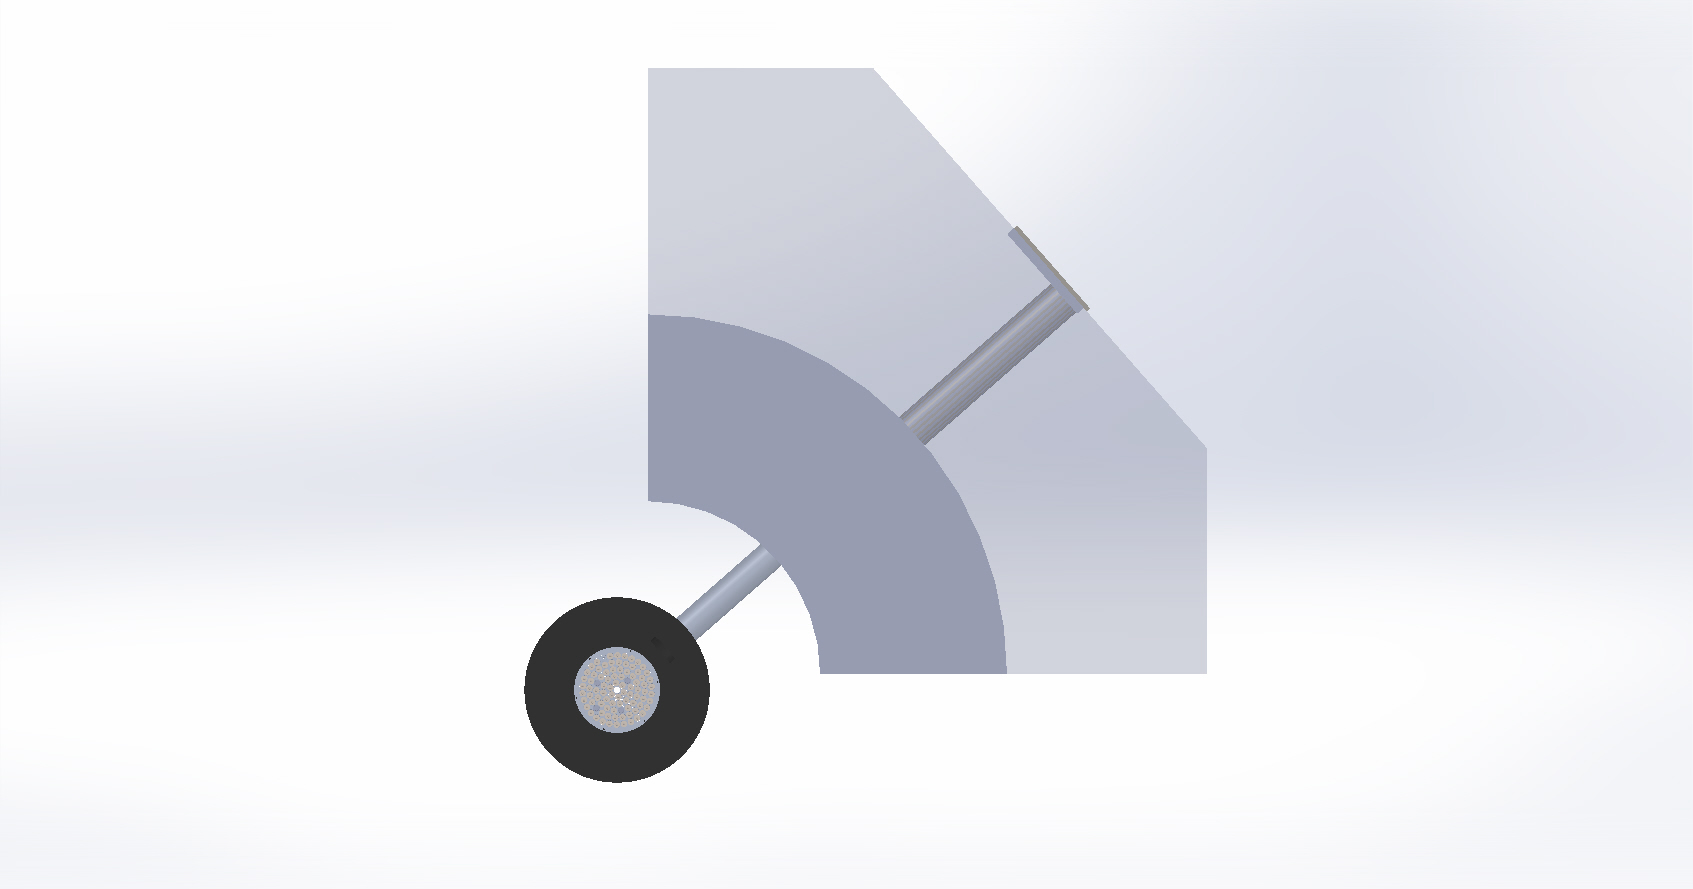
\includegraphics[height=3in]{tex/figures/solidworksxy.jpg}
\caption[Solidworks $XY$]{An $xy$ view of the quarter section of the reactor containing the NEBP.}
\label{fig:solidworksxy}
\end{figure}


The NEBP geometry is relatively simple.
% two sections 6 and 8 inch
It is comprised of two, six-foot, cylindrical segments; the inner and outer segments being 6" and 8" in diameter, respectively.
% coupled by shadow shield
A lead ``shadow shield" is at the junction of these two sections to help reduce the gamma component of the outgoing particle stream.
The shadow shield is 4'x4' and 4" thick and contains a hole through the center, through which the outer portion of the NEBP's 6" section extends.
% material
The walls of each section are made of aluminum 11/32" thick.
% wooden plugs but now empty
Originally, these sections contained removable wooden plugs that would dissallow neutron to stream through; however, water leaks in the beam caused damage to these plugs and at present they have been removed.

% collimator
Within the 8" section lives a collimator.
% who made it
This was designed by a KSU senior design team attempting to further constrain the neutron beam.
% describe design
The collimator is an aluminum tube of 0.75" ID and 1" OD.
An aluminum plate is affixed to this tube on the reactor side and contains a throughhole to maintain line of sight with the reactor core.
This allows borated polyethylene disks to be stacked around the collimator for the purpose of absorping neutrons that escape the beam.
The borated polyethylene extends the entire distance of the collimator. 


\subsection{How it was implemented in mcnp}
\subsection{Rotation of the model}


% ------------------------------------------------------------------------------
\section{KCODE to SDEF/Fission Rates}

% ------------------------------------------------------------------------------
\section{Application of ADVANTG}

% ------------------------------------------------------------------------------
\section{Tally Results}
